\chapter{Binary sequence representation}
\label{kap:kap2}

As we have shown in the previous section, bit vector can be used to solve various practical
problems. This chapter is dedicated to outlining the current state of the bit vector
implementations supporting methods $\access$, $\rank$ and $\select$. We start with a succinct
representation of bit vector and present ideas to support $\rank$ and $\select$ in sublinear
extra space. Then we look at the compressed representation of bit vector obtained using the
method introduced by \cite{raman2007succinct}.

\section{Bit vector implementation}

In this section, we introduce practical but also optimal constant time implementations of
$\rank$ and $\select$ methods with sublinear space overhead.

\subsection{Rank}
\label{section:rank}

Regarding $\rank$ in bit vector, we are concerned with two different methods, namely $\rank_0(i)$
and $\rank_1(i)$. In every binary sequence, it holds that $$\rank_0(i) = i - \rank_1(i).$$
Thus, it is common to only provide the implementation for one of them and answer the other one
using the formula above. Thus, from now on, we consider only $\rank_1(i)$ method and denote
it $\rank$ to simplify notation. There are two straightforward solutions we can begin with to
support $\rank$ on a bit vector~$B$.

The first solution does not use any precomputation at all. Every time we want
to compute $\rank(i)$, we go through all the bits preceding $i$-th and count all
the ones. This solution is not practical for long bit vectors but it does not require
any additional space and precomputation.

The second approach is to precompute $\rank$ of every bit, which enables us to answer
$\rank$ query in constant time, using a single table lookup. However, the space needed to
support this solution is $\BigO(n\cdot\log n)$ bits, where $n$ is the length of the
bit sequence.

Presented solutions can be combined to obtain an idea of a practically
interesting solution where the pre-computed $\rank$ values are stored only for some
bits. At first, we choose a constant $k$ and split bit vector into non-overlapping
subsequences of $k$ bits called \textit{superblocks}. We then precompute $\rank$ only for
the beginning of every superblock. Example of this representation is presented in
Fig.~\ref{obr:practicalRank}. This representation enables answering $\rank$ in time
$\BigO(k)$ as only the precomputed value is accessed and then bits from the start of the
superblock up to the queried position are accessed. This solution uses $\BigO(\ceil{n/k}\log n)$
bits of memory as there are $\ceil{n/k}$ superblocks and every rank stored is at most $n$,
thus taking $\BigO(\log n)$ bits. This version of the implementation allows us to balance between
speed and space usage using the parameter $k$. Increasing parameter $k$ saves space, on the other
hand, smaller $k$ requires less computation to be done inside of the superblock.

In practice, the time of answering the query for smaller $k$ may be dominated by cache miss
that often occurs when accessing $\rank$ precomputed for the superblock. Subsequent linear
scan through superblock is very cache-friendly and thus very fast.

% TODO: moreover, bit operations - popcount
% TODO: in theory, for k ~ log n we already get linear space and \BigO(1) time if we assume a strong-enough model (RAM with log n bit registers with popcount)

\begin{figure}
	\begin{tabular}{c|c|c|c|c|}
	\cline{2-5}
	\textbf{B} & {\tt 0 0 1 0 1 1 0 1} & {\tt 1 1 1 0 1 1 1 1} & {\tt 0 0 0 0 0 1 1 0} & {\tt 1 1 0 0 1} \\ \cline{2-5}
	\end{tabular}

    \bigskip

    \begin{tabular}{c|c|c|c|c|}
        \cline{2-5}
        \textbf{precomputed ranks} & \tt 0 & \tt 4 & \tt 11 & \tt 13 \\ \cline{2-5}
        \end{tabular}

	\caption[TODO]{Example of dividing bit sequence $B$ into superblocks of length 8 and precomputing
    $\rank_1$ for the beginning of every superblock. Note that last superblock may not contain full
    number of 8 bits.}
	\label{obr:practicalRank}
\end{figure}

\paragraph{Constant time rank with sublinear space overhead}

The previous solution works well and is commonly used in practice. However, it is possible to
answer $\rank$ query in constant time with only sublinear space overhead. The constant time
solution is based on work of \cite{jacobson1988succinct}. As in the previous solution, we start
by splitting the bit sequence into superblocks. This time we set the length of a superblock to
$\BigO(\log^2 n)$ and again precompute $\rank$s for the beginning of every superblock. Then, every
superblock is further subdivided into blocks of length $\ceil{(\log_2 n)/2}$. Similarly to superblocks,
for all of these smaller blocks, we precompute $\rank$. However, to save space, we only precompute
these $\rank$s from the beginning of the corresponding superblock.

Now, when queried for $\rank$ of some position $i$, we combine:
\begin{enumerate}
    \item $\rank$ precomputed for the beginning of its superblock, plus
    \item $\rank$ precomputed for the beginning of its block, plus
    \item $\rank$ inside of its block
\end{enumerate}

The third step can be done also in constant time on unit-cost RAM model with word size $\Theta(\log n)$
that we use in most of our work. In weaker models, we can still use a precomputed table. This table stores
for every possible block and $\rank$ query its result. 

The additional space used by this solution can be broken down into three parts:
\begin{enumerate}
    \item Precomputed $\rank$ for every superblock: The number of superblocks is $\BigO(n/\log^2 n)$
    and we need $\BigO(\log n)$ bits to store every single $\rank$ value so the total amount is
    \begin{equation}
        \BigO\left(\frac{n}{\log^2 n}\cdot \log n\right) = o(n).
        \label{eq:rank_space_1}
    \end{equation}
    \item Precomputed $\rank$ for every block: The number of smaller blocks is $\BigO(n/\log n)$. For every
    block, precomputed $\rank$ from the beginning of a superblock is stored. This value is at most $\log^2 n$,
    thus we need $\BigO(\log\log^2 n)=\BigO(\log\log n)$ bits to store it. The total amount of space is
    \begin{equation}
        \BigO\left(\frac{n}{\log n}\cdot \log\log n\right)=o(n).
        \label{eq:rank_space_2}
    \end{equation}
    \item Precomputed table storing result for every possible $\rank$ query over every possible block: There
    are only $\BigO(2^{(\log n)/2}) = \BigO(\sqrt{n})$ blocks of length $\BigO((\log n)/2)$. The number of
    possible $\rank$ queries over a block is equal to its length. For every element stored in the table we need
    at most $\BigO(\log\log n)$ bits of space so the total amount of space is
    \begin{equation}
        \BigO(\sqrt{n}\cdot \log n\cdot \log\log n)=o(n).
        \label{eq:rank_space_3}
    \end{equation}
\end{enumerate}

The total space used for this solution of $\rank$ is therefore a sum of \ref{eq:rank_space_1}, \ref{eq:rank_space_2}
and \ref{eq:rank_space_3}, which is sublinear in $n$.

Even if optimal in theory, this solution is not often used in practice as it involves a
quite complex implementation and produces 3 cache misses per query:  One for accessing the
precomputed rank up to the start of the superblock, then another one for the precomputed
value of rank to the beginning of the block and in the end also one for accessing the precomputed
$\rank$ value of the block.

% TODO: ... depends on model... can be \BigO(k/w) if we consider RAM model with w-bit registers
% that supports popcount

\subsection{Select}
\label{section:select}

In case of a $\select$ over bit vector, we are again interested in two methods $\select_0$
and $select_1$. Even if there is not a simple way how to convert the result of one to
another just like with $rank$, we shall be interested mainly in $select_1$ version as the
other one can be implemented using the same ideas. The important property of the $\select$
method is that it works much like an inverse to $\rank$. This is given by the fact that
$$\rank_c(\select_c(i)) = i.$$

Thanks to $\rank$ being a nondecreasing function, it is possible to binary search for the
result of $\select_c(i)$ if we have an efficient implementation of $\rank$. This can be combined
with the solution from the previous section. At first, we binary search for the solution in the
samples of $\rank$ stored in superblocks. After identifying the correct superblock of length $k$
bits, we linearly scan for the result. This solution does not require any additional memory on top
of the space used for $\rank$. The answer is computed in time $\BigO(\log(n/k)+k)$. Even though this
solution is not optimal, it works very well in practice, as observed by \cite{gonzalez2005practical}
on bit vectors of length up to $2^{20}\approx 10^6$.

\paragraph{Constant time select}

\cite{clark1997compact} proposed solution for $\select$ in constant time and sublinear space
overhead. The solution is, similarly to the constant time $\rank$ solution, based on a division
into blocks and superblocks.

We begin by precomputing $select(i)$ for every $i$ being multiple of $t_1=\log n\cdot \log\log n$.
These precomputed values take $\BigO(n/\log\log n)$ bits of space. Results of these precomputed
$\select$ queries split the bit sequence into superblocks of possibly variable length such that
each superblock contains exactly $t_1$ ones (except possibly for the last superblock).

There are now two categories of superblocks. The ones called \textit{long} that are longer
than $t_1^2$. In long superblocks, we can store the positions of all ones as they are sparse
and there are not many of these blocks. The total space used is $$\BigO((n/t_1^2)\cdot t_1\cdot
\log n) = \BigO(n/\log\log n),$$ which is still $o(n)$.

Dealing with \textit{short} superblocks is harder. On short superblocks, we apply the idea that we
already used for the original bit sequence. Inside of every short superblock, we precompute the
$\select$ from the beginning of the superblock for every multiple of $t_2=(\log\log n)^2$. These
precomputed values are small as they only represent positions from the beginning of a short superblock.
Each of these values takes $\BigO(\log\log n)$ of space so the total amount of space used by these
values is $\BigO(n/t_2\cdot \log\log n) = \BigO(n/\log\log n)$.

This procedure breaks short superblocks into blocks. Again, each of these blocks, possibly except for the
last one contains $t_2$ ones. For blocks longer than $t_2^2$, we store the positions of all
ones as there are not many of these blocks. We may use the same reasoning as in the previous
part to conclude that this takes $\BigO(n/t_2^2\cdot t_2\cdot \log\log n) = \BigO(n/\log\log n)$
bits.

To deal with the blocks smaller than $t_2^2$, we can again precompute a table of all
the possible ways how the block may look and all the possible $\select$ queries over it with
their result. The number of possible blocks of length $t_2^2$ is equal to $\BigO(2^{t_2^2})$,
the number of possible queries over the block is at most its length $t_2^2$ and to store the
results we need roughly $\BigO(\log t_2)$ bits. The table size is thus
$$\BigO(2^{t_2^2}\cdot t_2^2 \cdot \log t_2) = o(n).$$

When answering $select_1(i)$, we first find the location of the right superblock. If this
is a long superblock, we just look at the precomputed positions of ones in the superblock.
The matter is more complicated if we are dealing with a short superblock. In this case, we find
the location of the correct block. If this is a long block, we can once again just look
at the position of one we are interested in. If it is a short block, we use the precomputed
table.

\section{Compressed representation}
\label{section:compressed_bv}

In the previous section, we showed how $\rank$ and $\select$ queries can be answered in constant
time with just sublinear space overhead. In this section, we show that it is possible to compress
the whole bit vector close to the zeroth order entropy while still keeping the constant time $\rank$
and $\select$.

Up to now, we have been working with a straightforward representation of bit vector in which we store
all the bits one after another. This is the best we can do in general, but there are scenarios
where there is a room for improvement. One example is if the zeroth order entropy $H_0$ of a bit sequence
is small. This occurs in sequences that have a very skewed frequency of zeroes or ones. If sequence of
length $n$ has $m$ ones in it, we can store it as before using $n$ bits. There is, however, only ${n \choose m}$
such sequences and it may be more beneficial for small/big $m$ to store rather the sequence number which
one of these ${n \choose m}$ sequences we are working with. It is possible to prove for sequence $S$ of
length $n$ with $m$ ones that $$\lg {n \choose m} = nH_0(S)+\BigO(\log n).$$ This means that using this
representation may be beneficial in scenarios when $nH_0(S)\ll n$.

This is an idea that RRR is based on. RRR is a data structure based partly on the work of \cite{pagh2001low}
and proposed by \cite{raman2007succinct}. We split the bit sequence into blocks of length $b$ and then
represent a block with $c$ ones using only $\lg {b \choose c}$ bits as there are ${b \choose c}$ combinations
for positions of ones. The whole block can then be uniquely represented as a pair $(c, o)$ where $c$ is the
number of ones in the block, called \emph{class} and $o$ is an \emph{offset} of this block in a sequence of
all the ${b \choose c}$ blocks in this particular class. Even if the ordering of the blocks with the same class
can be arbitrary, only lexicographical ordering is heavily used in practice.

Now, for this structure to work, we need to find a way how to convert between the bit representation of
a block and its compressed form $(c, o)$. The process of obtaining $c$ and $o$ from the raw representation
of block is called \textit{encoding}. The opposite process is called \textit{decoding}. We would like both
processes to be fast, however, in most of the applications where bit vector is used, we do the encoding only
once at the initial construction of the bit vector. Decoding, on the other hand, is done every time we are
accessing a particular bit in $B$. Thus, in practice, it is more important to optimise the speed of decoding.

\paragraph{Block encoding/decoding}

For shorter block lengths, such as $b\leq 15$, it is reasonable to generate two helper tables $E$ and $D$.
Table $E$ used for the encoding, maps the block to its offset. The other table $D$ is two dimensional and
stores the bit representation of the block that is associated with pair $(c, o)$ on position $D[c][o]$.
Both these tables $E$ and $D$ can be precomputed by generating all the possible blocks in lexicographical
order. After this precomputation, the encoding and decoding of a block takes constant time.

For longer blocks, it is impractical or even impossible to store huge helper tables. On the other
hand, longer blocks yield better compression rates because of smaller per block overhead. \cite{navarro2012fast}
developed method we shall call \textit{on the fly-decoding}, that does not require these big helper tables. 
This method relies on a bit by bit encoding and decoding of the block, taking $\BigO(b)$ time. While decoding,
we can compute on every position, how many blocks precede a given prefix using simple combinatorics. Based on
that number, we decide whether next bit should be {\tt 0} or {\tt 1}. Pseudocode of this idea computing binary
representation of block is in listing~\ref{alg:on_the_fly}.

\begin{algorithm}
\caption{On-the-fly decoding}\label{alg:on_the_fly}
    \KwData{$c, o$}
    $block \gets 0$\;
    \For{$i=0$ \KwTo $b-1$} {
        \tcp{$p$ is the number of blocks with the same prefix  and zero on $i$-th position}
        $p \gets {b-i-1\choose c}$\;
        \If{$o<p$} {
            \tcp{add zero at the end of the block}
            $block \gets 2\cdot block$\;
        } \Else {
            \tcp{add one at the end of the block}
            $block \gets 2\cdot block+1$\;
            $c \gets c-1$\;
            $o \gets o-p$\;
        }
    }
    \KwRet{$block$}
\end{algorithm}

On the fly decoding does not use helper tables $E$ and $D$ but to achieve the best possible time complexity,
it requires the precomputation of Binomial coefficients it uses. These, however, use together less than $\BigO(b^3)$
of bits.

\paragraph{Arrangement of encoded blocks}

In the previous paragraph, we showed how a single block can be decoded. The next question is how the
encoded pairs representing blocks are arranged in memory. This arrangement should consider space efficiency
but also allow easy access to individual blocks of $B$.

The main part of this representation comprises of two arrays $C$ and $O$ storing the classes and offsets of
the blocks, respectively. The array $C$ is an array of elements that are of fixed length. Every element takes
$\lg (b+1)$ bits of space as the number of ones in the block can be anywhere between 0 and $b$. The array $O$,
on the other hand, is an array of elements of variable length where the $i$-th element is $\lg {b\choose C[i]}$
bits long where ${b\choose C[i]}$ is the number of blocks along the class $C[i]$. Note that accessing $i$-th element
in array $C$ is easier than doing the same in array $O$.

\paragraph{Accessing bits in RRR}

Accessing $x$-th bit of the original sequence $B$ consists of three steps. The first step is to obtain the
compressed representation of a block where $x$-th bit is located. The second step is to decode this block and
the third is to access the particular bit of interest in the decoded block. The $x$-th bit is contained in the
$i$-th block where $i=\floor{x/b}$. Its compressed representation is $(C[i], O[i])$ where $C[i]$ stands for class
and $O[i]$ for the offset along the all possible blocks with class $C[i]$.

Obtaining $C[i]$ is trivial as it is at the fixed memory offset from the beginning of array $C$. Getting the
value of $O[i]$ is harder as it is not at a known memory offset but this memory offset can be expressed as
$$\sum_{j=0}^{i-1} \lg {b\choose C[j]}$$, where we basically sum up the lengths of all the elements preceding
$O[i]$. This can not be, however, computed in constant time without any precomputed information and we
need to basically one by one skip over elements that come before $O[i]$. To access the $i$-th block without
precomputed information, we need in the worst case to look at all the elements of $C$ and this takes $\BigO(n/b)$
time. For now, let us analyze space usage of this solution.

\paragraph{Space usage of RRR}

Our current representation needs to store the arrays $C, O$. Let us now analyze the space used by these structures.
Array of classes $C$ is an array of $\ceil{n/b}$ elements of fixed length $\lg (b+1)$. For offset array $O$ we argue
that its size is bounded by
\begin{align*}
    \sum_{i=1}^{n/b} \lg {b\choose c_i}
    &\leq \sum_{i=1}^{\ceil{n/b}} \log_2 {b\choose c_i} + \ceil{n/b} \\
    &= \log_2\prod_{i=1}^{\ceil{n/b}} {b\choose c_i} + \ceil{n/b} \\
    &\leq \log_2{n\choose \#_1(B)} + \ceil{n/b} &\leq nH_0(B) + \ceil{n/b}
\end{align*}
where $\#_1(B)$ denotes the total number of ones in $B$. The second inequality was obtained using
the observation that ${n\choose k} {m\choose \ell} \leq {n+m\choose k+\ell}$. This can be seen
when we interpret the left side as the number of ways we can choose $k$ elements
from $n$ elements and $\ell$ elements from another $m$ elements. Any such choice is included in the
right side, which represents choices of $k+\ell$ elements from $n+m$. To understand the last inequality,
consider all binary sequences of length $n$ with $m$ ones. There are ${n\choose m}$ such sequences,
thus in the worst case, the space we need to represent a single one of these sequences is equal to
\begin{align*}
    \lg{n\choose m}
    &= n\log_2 n - m\log_2 m - (n-m)\log_2 (n-m) - \BigO(\log n) \\
    &= m\log_2 n + (n-m)\log_2 n - m\log_2 m - (n-m)\log_2 (n-m) - \BigO(\log n) \\
    &= n\left(\frac{m}{n}\log_2\frac{n}{m} + \frac{n-m}{n}\log_2\frac{n}{n-m}\right)-\BigO(\log n) \\
    &= nH_0(B) - \BigO(\log n).
\end{align*}

If we choose the decoding method with a helper table,  $D$ is storing $2^b$ entries and each entry takes
$b$ bits of storage. To summarize, the total space used is then
$$nH_0(B) + \ceil{n/b} + \ceil{n/b} \cdot \lg(b+1) + b2^b.$$

\paragraph{Block access speed up}

To speed up the process of accessing blocks, we can store pointers to every $k$-th element
of $O$. This again creates some bigger superblocks as can be observed in Fig.~\ref{obr:RRRFinal}.
This representation speeds up the process of locating offset $O[i]$. Now, we first find the
nearest pointer leading to superblock where $i$ is located and then we just skip through the superblock
at most $k$ times to locate $O[i]$. This additional structure of $\floor{n/(bk)}$ integers uses
$\BigO(\log(n)\cdot \frac{n}{bk})$ bits of space.

\begin{figure}
	\centerline{
		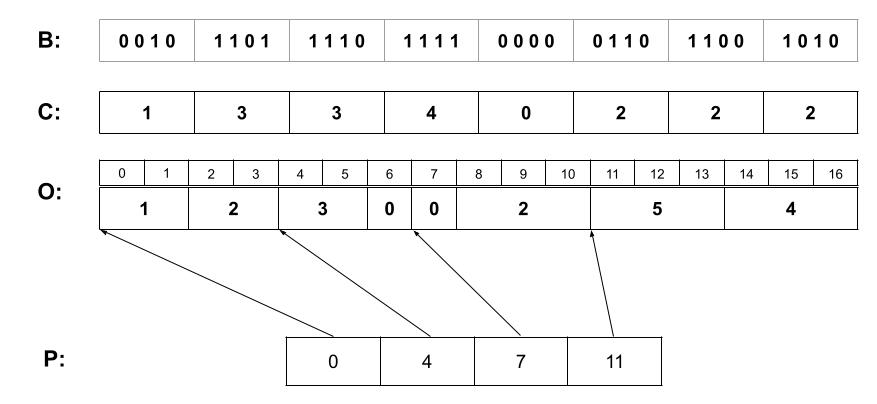
\includegraphics[width=0.9\textwidth, height=0.3\textheight]{images/rrr}
	}
	\caption[TODO]{RRR implementation. $B$ shows the original bit sequence cut to
    blocks. $C$ stores the class which is in this case number of ones in the block.
    $O$ uses variable number of bits per entry, in general, $i$-th entry uses
    $\lg {b\choose C[i]}$ bits and stores the lexicographical order
    of this block in the class $C[i]$. For $k=2$, we can see a helper array $P$
    storing bit offsets into every $k$-th element namely $0, 2, 4\ldots$
	}
	\label{obr:RRRFinal}
	% source at https://docs.google.com/drawings/d/1f1M7e-dZIiIZh1RdgqnmptF3xWZBKqjms3f_aQwVMhg/edit
\end{figure}

When setting the block length to $\log(n)/2$, we obtain interesting practical results as
the total space used by our representation is equal to $nH_0(B) + o(n)$ bits. This means
that we are storing only a sublinear amount of data on top of the zeroth order empirical entropy.

When we are interested in obtaining the best practical results, block length becomes
one of the most important parameters of RRR implementation. As we shall show in the Chapter
4, longer blocks yield lower per bit overhead. Also, not all block
lengths are used in practice. Very often, we are interested in block lengths of the form $2^k-1$.
This is because the number of ones in block of length $2^k-1$ can be number between 0 and $2^k-1$
making this in total $2^k$ possibilities. Storing this number in the fixed bucket of size
$k$ bits makes use of all the available space. This is why most commonly used bucket sizes in
practice are 4, 5, 6 and 7 for block lengths 15, 31, 63 and 127.

For block length of 15, the encoding and decoding table each occupies roughly 64kB of space. This
is because each table consists of $2^{15}$ entries each taking 2 bytes of storage. Unfortunately,
for block length of 31, these two tables would consume roughly $2^{31}\cdot 4$ bytes of storage. That
amounts to roughly 8.5GB of space and makes this approach unusable in practice. This problem forces us
to use the on the fly decoding for block lengths bigger than 15. The disadvantage of this approach is
that it takes $\BigO(b)$ steps to decode the block. Furthermore, on the fly decoding contains branches
and it is hard to parallelize its steps in some meaningful way. Overall, this makes the block length a
parameter that we can adjust to balance between better space efficiency and faster runtime performance.